\chapter{SSL, TLS e Certificati}

SSL (Secure Sockets Layer) e TLS (Transport Layer Security) sono lo stesso 
tipo di protocolli con algoritmi crittografici diversi; assicurano che la comunicazione
tra due host avvenga in un \textbf{canale sicuro}, facendo rispettare \textbf{integrità}
e \textbf{autenticità}. 

\begin{figure}[H]
    \centering
    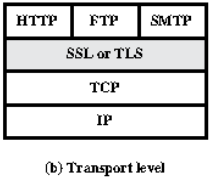
\includegraphics[width=0.4\linewidth]{chapters/10/images/intro.png}
\end{figure}

\noindent Vengono impiegati in ogni browser web, sistemi di pagamento, \dots

\section{SSL \textit{basics}}
SSL consiste in diversi protocolli:
\begin{itemize}
    \item \textbf{Handshake protocol:} usa chiave pubbliche per stabilire le chiavi 
    segrete condivise tra client e server 
    \item \textbf{Record protocol:} fornisce dei servizi di sicurezza ai protocolli di livello 
    più alto; usa le chiavi segrete per proteggere la confidenzialità, integrità e autenticità
    dei dati
    \item si \textit{negozia la versione del protocollo e gli algoritmi 
    crittografici da usare}
    \item \textit{autentica server e client} (opzionale); vengono usati dei certificati
    digitali per verificare le identità (spesso solo il server è autenticato)
\end{itemize}

\section{TLS \textit{basics}}
TLS si pone tra il livello applicativo e quello di trasporto: i dati non protetti 
vengono forniti a TLS, che li trasforma in dati criptati per poi fornirli al livello 
sottostante (trasporto).

\begin{figure}[H]
    \centering
    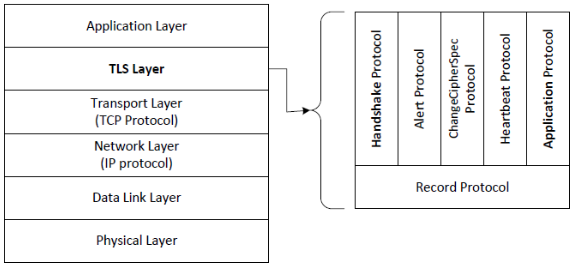
\includegraphics[width=1\linewidth]{chapters/10/images/tls-basics.png}
\end{figure}

\noindent In TLS ci sono \textit{due entità} principali:
\begin{itemize}
    \item \textbf{Connessione:} un trasporto che fornisce un tipo di servizio adeguate; in TLS, 
    tali connessioni sono relazioni \textit{peer-to-peer} (i nodi sono equivalenti)

    \noindent Ogni connessione è transitoria ed è associata ad una sessione
    \item \textbf{Sessione:} è un'associazione tra client e server creata dal protocollo di handshake;
    ogni sessione definise dei parametri crittografici di sicurezza che possono 
    essere condivisi tra più connessioni
    
    $\rightarrow$ vengono utilizzate per evitare la costosa negoziazione 
    di nuovi parametri di sicurezza per ogni connessione
\end{itemize}

\noindent Tra qualsiasi coppia di parti (ad esempio applicazioni come HTTP su client 
e server) potrebbero esserci più connessioni protette (in teoria anche più sessione,
ma non accade nella pratica).

\subsection{Componenti di TLS}

\subsubsection{Alert Protocol}
Notifica situazioni anomale o segnala eventuali problemi; viene usato per 
trasmettere allarmi relativi al protocollo SSL/TLS all'altra entità in 
comunicazione. Ogni messaggio è compsoto da \textbf{2 byte}:
\begin{itemize}
    \item il \textit{primo byte} assume il valore di \textbf{warning} o \textbf{fatal}
    che indica la gravità del messaggio identificato dal secondo byte; i messaggi \textit{fatal}
    sono irreversibili e la sessione viene interrota
    \item il \textit{secondo byte} contiene un codice che indica l'\textbf{avviso specifico}
\end{itemize}

\subsubsection{Handshake protocol}
Permette alle parti di negoziare i diversi algoritmi necessari per la sicurezza 
della comunicazione, consente l'eventuale autenticazione e lo scambio delle chiavi.

\noindent È fatto da una sequenza di messaggi, ciascuno dei quali ha i 
seguenti campi:
\begin{itemize}
    \item \textbf{Tipo} (1 byte): indica uno dei 10 tipi di messaggi disponibili
    \begin{itemize}
        \item \texttt{hello\_request}
        \item \texttt{client\_hello}
        \item \texttt{server\_hello}
        \item \texttt{certificate\_request}
        \item \texttt{certificate}
        \item \texttt{certificate\_verify}
        \item \texttt{server\_key\_exchange}
        \item \texttt{clinet\_key\_exchange}
        \item \texttt{server\_done}
        \item \texttt{finished}
    \end{itemize}
    \item \textbf{Lunghezza} (3 byte)
    \item \textbf{Contenuto} (byte): i parametri associati al messaggio
\end{itemize}

\begin{figure}[H]
    \centering
    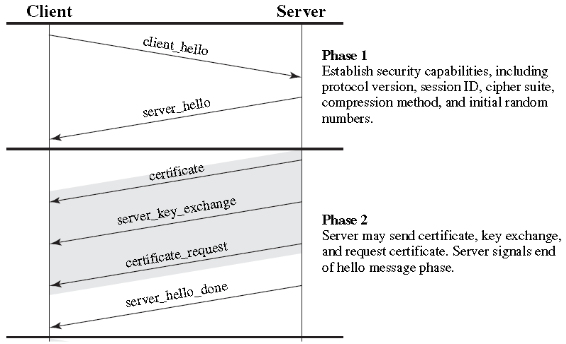
\includegraphics[width=1\linewidth]{chapters/10/images/hs1.png}
\end{figure}
\begin{figure}[H]
    \centering
    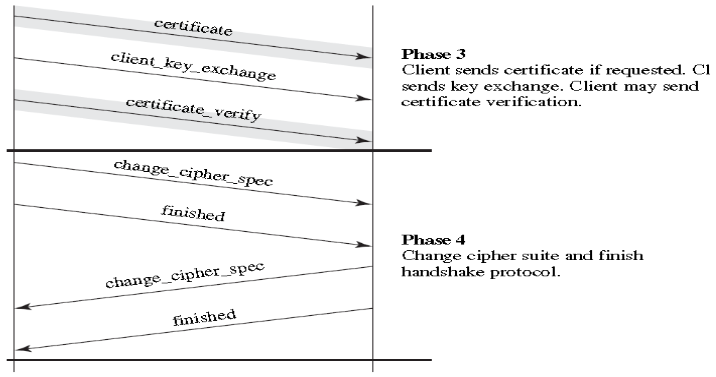
\includegraphics[width=1\linewidth]{chapters/10/images/hs2.png}
\end{figure}

\noindent La \textbf{generazione} e \textbf{scambio delle chiavi} viene fatta
in tre passaggi:
\begin{itemize}
    \item \textit{Segreto pre-master}: viene crittografato un numero casuale con la chiave pubblica del server 
    \item \textit{Segreto master}: viene generato usando i \textit{nonce} scambiati durante l'handshake e il 
    segreto pre-master 
    \item \textit{Chiave di sessione}: viene usato il segreto principale per generare 
    una sequenza di byte (le chiavi, dipendono dall'algortimo di cifratura)
\end{itemize}


\subsubsection{Change chiper spec protocol}
Impone l'esecuzione di un nuovo handshake per rinegoziare i parametri di sicurezza 
e ripetere l'autenticazione. 

\noindent È costituito da un singolo byte impostato al valore 1.

\subsubsection{Record protocol}
Fornisce \textit{due servizi} per le connessioni TLS:
\begin{itemize}
    \item \textbf{confidenzialità:} usa la chiave segreta condivisa durante l'handshake
    \item \textbf{integrità dei messaggi:} la stessa chiave segreta viene usata per il MAC (Message 
    Authentication Code)
\end{itemize}

I passagi che segue il protocollo sono:
\begin{enumerate}
    \item prende in input un messaggio da trasmettere 
    \item frammenta l'input in blocchi 
    \item applica il MAC al frammento (lo concatena in coda)
    \item cifra quanto ottenuto 
    \item aggiunge un'intestazione e trasmette in un segmento TCP; l'header contiene:
    \begin{itemize}
        \item \textit{content-type} (alert, handshake, \dots)
        \item \textit{versione}
        \item \textit{lunghezza del payload}
    \end{itemize}
\end{enumerate}

\begin{figure}[H]
    \centering
    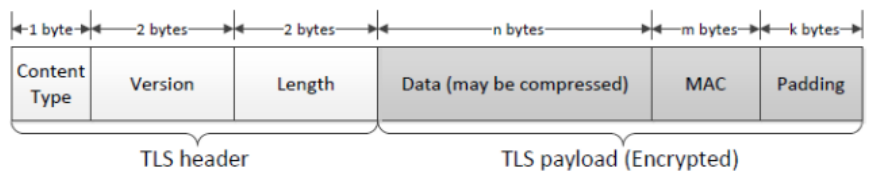
\includegraphics[width=1\linewidth]{chapters/10/images/tls-record.png}
\end{figure}

\subsection{Stato di sessioni e connessioni}

Lo stato di una sessione è definito da:
\begin{itemize}
    \item \textbf{identificatore}
    \item \textbf{certificato peer}
    \item \textbf{metodo di compressione} (da TLS 1.3 è vietato comprimere)
    \item \textbf{cipher spec:} algoritmo di crittografia usato e una funzione di hash da usare per il MAC 
    \item \textbf{master secret}
    \item \textbf{\texttt{isResumable}:} una flag che indica se è possibile avviare nuove connessioni dalla sessione
\end{itemize}

\noindent Lo stato di una connessione è definito da:
\begin{itemize}
    \item \textbf{server e client randomness} (sequenza di byte)
    \item \textbf{server write MAC secret}
    \item \textbf{client write MAC secret}
    \item \textbf{chiave di scrittura server}
    \item \textbf{chiave di scrittura client}
    \item \textbf{numeri di sequenza} 
\end{itemize}

\subsection{Costo di una sessione}
Sia lato client che lato server:
\begin{itemize}
    \item generare valori casuali 
    \item verifica dei certificati
    \item cifrare/decifrare i valori casuali con la chiave opportuna
    \item calcolare chiave con hash 
\end{itemize}

\noindent $\rightarrow$ ogni sessone ha un costo elevato; tanto richieste di connessione 
potrebbero portare ad un DoS

\section{SSH (Secure Shell)}
SSH è un protocollo di rete crittografico che permette di stabilire una sessione remota cifrata tramite interfaccia a riga di comando con un altro host di una rete informatica.

\noindent SSH è organizzato come tre protocolli che tipicamente vengono eseguiti su TCP:
\begin{itemize}
    \item \textbf{Transport Layer Protocol:} fornisce l'autenticazione del server, la riservatezza e l'integrità
    dei dati 
    \item \textbf{Protocollo di autenticazione utente} per autenticare l'utente sul server
    \item \textbf{Protocollo di connessione}
\end{itemize}

\noindent Sia TLS che SSH creano un tunnel per il trasporto di dati sicuro; hanno però alcune
differenze relative alla sua realizzazione, come i formati usati; inoltre, SSH ha dei protocolli 
per gestire ciò che accade all'interno del tunnel.


\section{Vulnerabilità}

\subsection{SSL \textit{version rollback}}
Il server viene ingannato pensando che sta comunicando con un client che 
supporta solo la versione SSL 2.0; questo è problematico perché:
\begin{itemize}
    \item le \textit{cipher spec} non sono autenticate 
    \item i messaggi dell'handshake non sono protetti 
    \item non supporta catene di certificazione
    \item \dots
\end{itemize}

\subsection{Man In The Middle TLS \textit{downgrade}}
Un utente malintenzionato che ha il controllo del traffico può simulare 
questo attacco ancora oggi.

Per gestire la connessione tra due dispositivi su una rete locale, bisogna 
fare in modo di reindirizzare il traffico attraverso l'attaccante, \textbf{manipolando 
la cache di ARP} (Address Resolution Protocol).

\section{HTTPS}
HTTPS è la versione sicura di HTTP; usa un canale sicuro SSL/TLS per inviare dei 
messaggi HTTP.

\noindent Bisogna fare attenzione che un attaccante non si introduca nel passaggio 
automatico tra HTTP e HTTPS: l'attaccante potrebbe redirizionare il traffico, 
intercettando i pacchetti della vittima e modificando la richiesta. 

\noindent La contromisura adottata è che le interazioni devono avvenire interamente 
in HTTPS; il browser si rifiuta di usare HTTP.

\section{Certificati}
I certificati in ambito web vengono rilasciati da un'ente accreditato a:
\begin{itemize}
    \item browser
    \item siti web
\end{itemize}

$\rightarrow$ prima di chiedere la pagina di un sito web, il browser richiede al web 
server il suo certificato; solamente dopo aver verificato chiede la pagina.

\noindent Un possibile attacco è quando un attaccante chiede un certificato legittimo
e ne crea una \textbf{copia falsa}, da usare ad esempio in un attacco di phishing.

\noindent Diventa fondamentale poter \textbf{revocare certificati}, ad esempio 
a causa di:
\begin{itemize}
    \item chiave privata compromessa 
    \item l'utente ha smesso di pagare per avere una certificazione, o non vuole più averla
    \item certificato compromesso
\end{itemize}

